\hypertarget{normative-decision-theory}{%
\section{Normative Decision Theory}\label{normative-decision-theory}}

The \textbf{normative decision theory is more rational}. E.g. if you
want to a maximum of profit and you have the options to open a store
with 125,000 CHF profit and another store with 150,000 CHF profit, you
decide for the second one \textbf{on a rational basis}.

The \textbf{main subject} of the normative decision theory is not
conflicting target but rather \textbf{uncertainty} (ger: Ungewissheit).

\hypertarget{result-decision-matrix}{%
\subsection{Result / Decision Matrix}\label{result-decision-matrix}}

The mineral oil company is aware that a large-scale bypass is planned
but that this is highly controversial. - It wouldn't affect the traffic
in the town centre and the expected profit would remain at CHF 125,000.
- However, there would be a drastic change to the outskirts of town
which would bring the expected profit down to CHF 80,000.

\textbf{Rresults matrix:} The form of depiction for decisions involving
uncertainty, where the alternativ actions (ai) are depicted in the rows
and the different environmental conditions in the columns (zi).

\begin{figure}
\centering
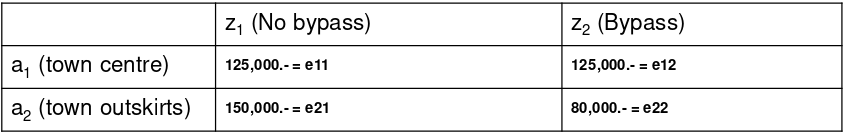
\includegraphics{figures/resultMatrix.png}
\caption{Results Matrix}
\end{figure}

The decision matrix only describes the decision situation if the state
space is recorded in full. So if there are changes on the environment in
future, you can not involve that in your decision.

\hypertarget{decision-with-probabilities}{%
\subsection{Decision with
probabilities}\label{decision-with-probabilities}}

\textbf{Decision involving risk:} If occurrence likelihoods can be
assigned to environmental conditions. \textbf{Decision involving
uncertainty:} If no occurrence likelihoods can be assigned to
environmental conditions.

\emph{Probabilitis must not only be mathematically or statistically
sound (objective probabilities), but rather may also only result from
the subjective view of the decision maker (subjective probabilities).}

\begin{figure}
\centering
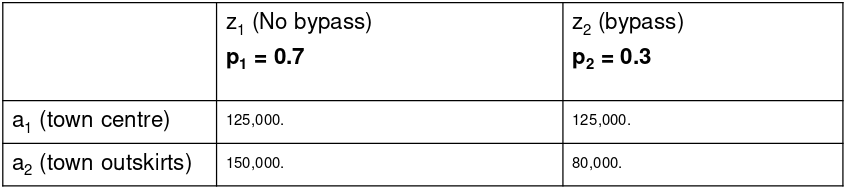
\includegraphics{figures/resultMatrix2.png}
\caption{Results Matrix}
\end{figure}

\hypertarget{dominance}{%
\subsection{Dominance}\label{dominance}}

An alternative is described as \textbf{dominant} if it is to be
preferred over another alternativ in all cases. If an alternative
dominates all others, it must be preferred on rational grounds.

\textbf{Absolute dominance}: If the worst result value of the dominating
alternative is better than the best result value of the dominating
alternative.

\textbf{Circumstantial dominance}: One alternative in every circumstance
(environmental circumstance) is better than (or equally good as) the
other alternative.

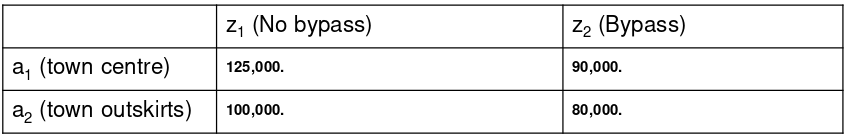
\includegraphics{figures/absoluteDominance.png} \emph{In this figure,
there is no absolute dominance, because a1 is not better in every
situation than the best of a2. There is no circumstantial dominance,
because a1 is better, regardless of the environmental conditions.}

\textbf{Target dominance}: If a target is considered to be a decisiv
one, the fulfilment of all other targets can be put aside.

\hypertarget{different-target}{%
\subsubsection{Different Target}\label{different-target}}

\begin{itemize}
\tightlist
\item
  \textbf{Complementary targets}: By pursuing one target, the other
  target is also (optimally) achieved.
\item
  \textbf{Neutral targets}: Don't influence each other.
\item
  \textbf{Competing targets}: Realising one target impacts on reaching
  the other target.
\end{itemize}

\hypertarget{lexiocographical-order}{%
\subsection{Lexiocographical order}\label{lexiocographical-order}}

In lexiocographical order you put priorities to some criterias
(e.g.~first priority = Sales, second priority = Environmental damage).
All options will be sorted according to the priorities (primary key and
secondary key) and the one on the top wins.

\hypertarget{utility-function-nutzwertanalyse}{%
\subsection{Utility function
(Nutzwertanalyse)}\label{utility-function-nutzwertanalyse}}

Weigthns the different parameters (e.g.~the factor for profit is higher
than for revenue). Afterwards the variant with the biggest utility is
the one to be choosen.

\hypertarget{decission-rules}{%
\subsection{Decission rules}\label{decission-rules}}

\hypertarget{maximin-rule}{%
\subsubsection{Maximin rule}\label{maximin-rule}}

The alternative action with the maximum minimum is chosen.

\textbf{Intention:} Decision rule with an extreme level of risk
aversion, as only the poorest possible result is reflected in the
evaluation.\\
\textbf{Criticism:} Not in touch with reality and only one single value
of an alternative is taken into consideration.

\hypertarget{maximax-rule}{%
\subsubsection{Maximax rule}\label{maximax-rule}}

The alternative action with the maximum maximum is chosen.

\textbf{Intention:} Extremely venturesome (optimistic) decision rule, as
only the best possible result is reflected in the evaluation.
\textbf{Criticism:} Extremely out of touch with reality and equally only
one single value of an alternative is taken into consideration.

\hypertarget{hurwicz-rule}{%
\subsubsection{Hurwicz rule}\label{hurwicz-rule}}

Combination of the maximin and maximax by the introduction of an
optimisation parameter lambda (0 \textless{}= lambda \textless{}= 1).

In optimistic decission making lambda should be choosen high, otherwise
it should be low.

\begin{figure}
\centering
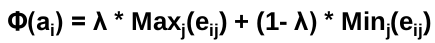
\includegraphics{figures/hurwicz.png}
\caption{hurwicz formula}
\end{figure}

\textbf{Intention:} Decision rule for decision makers who are neither
absolutely optimistic nor absolutely pessimistic. \textbf{Criticism:} In
many cases out of touch with reality and only two values of each
alternative are taken into consideration.

\hypertarget{savage-niehans-rule}{%
\subsubsection{Savage-Niehans rule}\label{savage-niehans-rule}}

Rule of the lowest regret.

The rule attempts to minimise the maximum possible regret. Create a
regret matrix matrix in which the maxima determine the environmental
conditions and then the maximum possible difference for this value is
calculated per course of cation. The maximum possible regret is then the
row maximum.

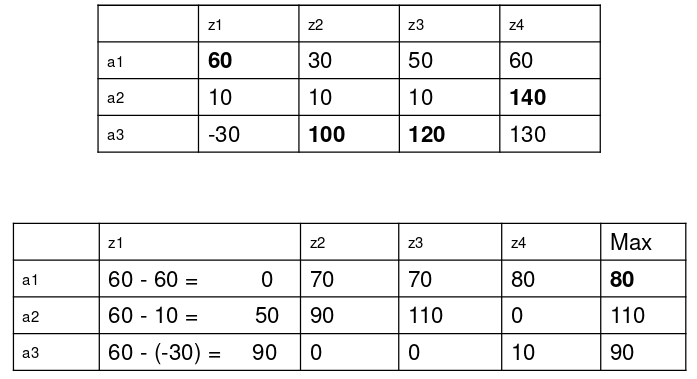
\includegraphics{figures/savage-niehansRule.png} You do following for
each column: Take the maximum value and calculate the possible lost
value for each cell. The row (alternative) with the minimum possible
lost value (the minimum regret) wins.

\textbf{Criticism:} With regard to the regret matrix, the decision is
based on the principles of the minimax criterion. For this reason, not
all information is used even in the case of this criterion and a
pessimistic sentiment is ultimately expressed. A particular point of
criticism relates to the circumstance that the ranking between two
alternatives can change after the addition of another alternative.

\hypertarget{laplace-criterion}{%
\subsubsection{Laplace criterion}\label{laplace-criterion}}

The average of all environmental conditions is formed for every
alternative. The winner is the alternative with the highest average over
all conditions.

\textbf{Criticism:} It can be said that probably most people would have
chosen the alternative a 3, and thus comparing the Laplace criterion
with the other rules is more realistic.

\hypertarget{logical-procedure}{%
\subsection{Logical procedure}\label{logical-procedure}}

Subjective probabilities for environmental conditions are formed and the
decision situation is converted in this way to a decision involving
risk.

\begin{figure}
\centering
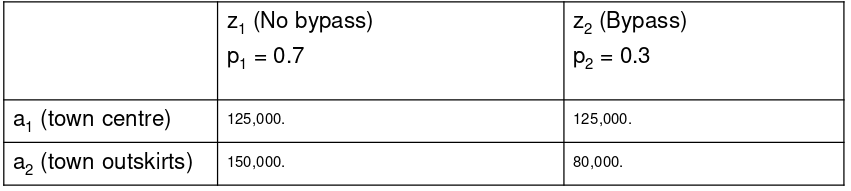
\includegraphics{figures/logicalDecisionMaking.png}
\caption{Decision involving risk}
\end{figure}

\hypertarget{mu-criterionbayes-rule}{%
\subsubsection{mu criterion/Bayes rule}\label{mu-criterionbayes-rule}}

\textbf{Expected value:} The expected value is the value which results
as a mean if the situation were to be endlessly repeated.

\begin{figure}
\centering
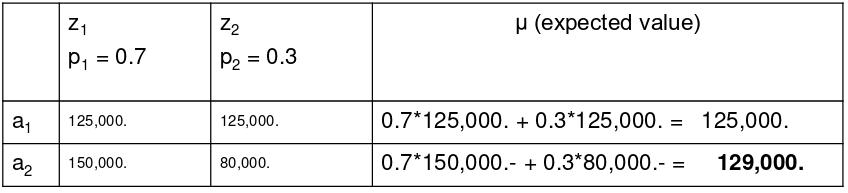
\includegraphics{figures/bayesRule.png}
\caption{Bayes rule}
\end{figure}

\textbf{risk aversion:} The decision maker prefers a lower expected
value if this provides more security.\\
\textbf{risk neutral:} The decision maker is indifferent to the
fluctuation of results, he only orientates himself on the expected
value.\\
\textbf{venturesome:} The decision maker avoids a higher expected value
in favour of a wide range of varying results.

\hypertarget{decission-tree}{%
\subsection{Decission Tree}\label{decission-tree}}

A decision tree always consists of one root node and any number of inner
nodes as well as at least two leaf nodes. Each node represents a logical
rule and each leaf node an answer to the decision problem.

\begin{verbatim}
Decisions are drawn in square fields. Events are drawn in circles. You can also note the probability of the alternative to the related leaf or the path.
\end{verbatim}

\hypertarget{bernoulli-principle}{%
\subsection{Bernoulli Principle}\label{bernoulli-principle}}

The basic idea is to calculate the expected value not from the results
values but rather from the utility values and to then regard these as
preferential values.\\
E.g. if you get a million CHF, you can do a lot of things! But if you
earn another million (=2 MIO), you can not do the double of these
things.

The Bernoulli survey can be used to determine the utility function,
which results in a risk-utility function (RNF) or a utility function.
The blue is risk neutral, the green is risky, the red is risk averse.

\begin{figure}
\centering
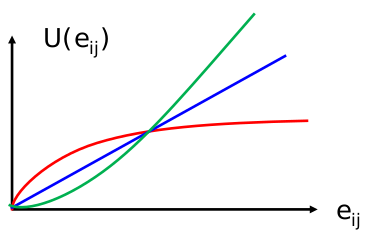
\includegraphics{figures/utilityFunction.png}
\caption{Utility Function}
\end{figure}

Procedure

If the risk utility function is given, a utility or decission marix can
be formed.

\begin{figure}
\centering
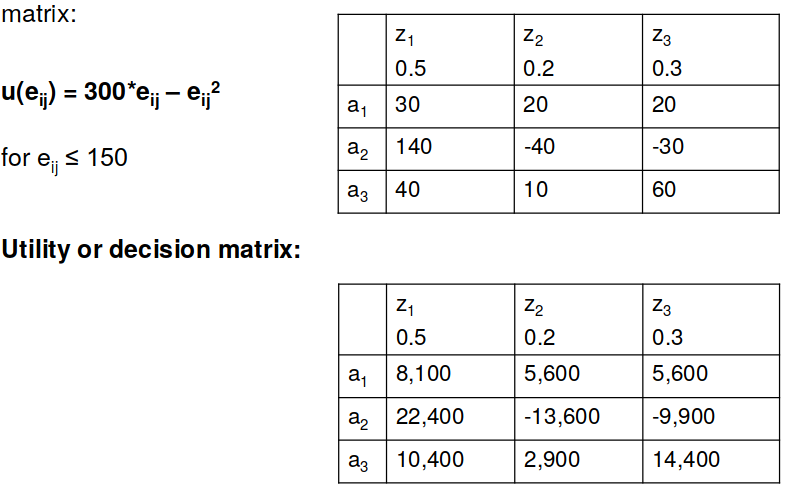
\includegraphics{figures/utilitymatrix.png}
\caption{Utility Matrix}
\end{figure}

If a risk utility function is given there's only \textbf{one rational
decission}.
